%%%%%%%%%%%%%%%%%%%%%%%%%%%%%%%%%%%%%%%%%
% Structured General Purpose Assignment
% LaTeX Template
%
% This template has been downloaded from:
% http://www.latextemplates.com
%
% Original author:
% Ted Pavlic (http://www.tedpavlic.com)
%
% Note:
% The \lipsum[#] commands throughout this template generate dummy text
% to fill the template out. These commands should all be removed when 
% writing assignment content.
%
%%%%%%%%%%%%%%%%%%%%%%%%%%%%%%%%%%%%%%%%%

%----------------------------------------------------------------------------------------
%	PACKAGES AND OTHER DOCUMENT CONFIGURATIONS
%----------------------------------------------------------------------------------------

\documentclass{article}

\usepackage{fancyhdr} % Required for custom headers
\usepackage{lastpage} % Required to determine the last page for the footer
\usepackage{extramarks} % Required for headers and footers
\usepackage{graphicx} % Required to insert images
\usepackage{caption}
\usepackage{float}
\usepackage{url}
\usepackage{subcaption}


% Margins
\topmargin=-0.45in
\evensidemargin=0in
\oddsidemargin=0in
\textwidth=6.5in
\textheight=9.0in
\headsep=0.25in 


\linespread{1.1} % Line spacing

% Set up the header and footer
\pagestyle{fancy}
\lhead{\hmwkAuthorName} % Top left header
\chead{\hmwkClass\ \hmwkTitle} % Top center header
\rhead{\firstxmark} % Top right header
\lfoot{\lastxmark} % Bottom left footer
\cfoot{} % Bottom center footer
\rfoot{Page\ \thepage\ of\ \pageref{LastPage}} % Bottom right footer
\renewcommand\headrulewidth{0.4pt} % Size of the header rule
\renewcommand\footrulewidth{0.4pt} % Size of the footer rule

\setlength\parindent{0pt} % Removes all indentation from paragraphs

%----------------------------------------------------------------------------------------
%	DOCUMENT STRUCTURE COMMANDS
%	Skip this unless you know what you're doing
%----------------------------------------------------------------------------------------

% Header and footer for when a page split occurs within a problem environment
\newcommand{\enterProblemHeader}[1]{
\nobreak\extramarks{#1}{#1 continued on next page\ldots}\nobreak
\nobreak\extramarks{#1 (continued)}{#1 continued on next page\ldots}\nobreak
}

% Header and footer for when a page split occurs between problem environments
\newcommand{\exitProblemHeader}[1]{
\nobreak\extramarks{#1 (continued)}{#1 continued on next page\ldots}\nobreak
\nobreak\extramarks{#1}{}\nobreak
}

\setcounter{secnumdepth}{0} % Removes default section numbers
\newcounter{homeworkProblemCounter} % Creates a counter to keep track of the number of problems

\newcommand{\homeworkProblemName}{}
\newenvironment{homeworkProblem}[1][Problem \arabic{homeworkProblemCounter}]{ % Makes a new environment called homeworkProblem which takes 1 argument (custom name) but the default is "Problem #"
\stepcounter{homeworkProblemCounter} % Increase counter for number of problems
\renewcommand{\homeworkProblemName}{#1} % Assign \homeworkProblemName the name of the problem
\section{\homeworkProblemName} % Make a section in the document with the custom problem count
\enterProblemHeader{\homeworkProblemName} % Header and footer within the environment
}{
\exitProblemHeader{\homeworkProblemName} % Header and footer after the environment
}

\newcommand{\problemAnswer}[1]{ % Defines the problem answer command with the content as the only argument
\noindent\framebox[\columnwidth][c]{\begin{minipage}{0.98\columnwidth}#1\end{minipage}} % Makes the box around the problem answer and puts the content inside
}

\newcommand{\homeworkSectionName}{}
\newenvironment{homeworkSection}[1]{ % New environment for sections within homework problems, takes 1 argument - the name of the section
\renewcommand{\homeworkSectionName}{#1} % Assign \homeworkSectionName to the name of the section from the environment argument
\subsection{\homeworkSectionName} % Make a subsection with the custom name of the subsection
\enterProblemHeader{\homeworkProblemName\ [\homeworkSectionName]} % Header and footer within the environment
}{
\enterProblemHeader{\homeworkProblemName} % Header and footer after the environment
}
   
%----------------------------------------------------------------------------------------
%	NAME AND CLASS SECTION
%----------------------------------------------------------------------------------------

\newcommand{\hmwkTitle}{"Fishing Association Website Prototype Development"} % Assignment title
\newcommand{\hmwkDueDate}{Tuesday,\ April\ 22,\ 2014} % Due date
\newcommand{\hmwkClass}{CS\ 22310} % Course/class
\newcommand{\hmwkAuthorName}{James Euesden - jee22} % Your name

%----------------------------------------------------------------------------------------
%	TITLE PAGE
%----------------------------------------------------------------------------------------

\title{
\vspace{2in}
\textmd{\textbf{\hmwkClass:\ \hmwkTitle}}\\
\normalsize\vspace{0.1in}\small{Due\ on\ \hmwkDueDate}\\
\vspace{3in}
}

\author{\textbf{\hmwkAuthorName}}
\date{} % Insert date here if you want it to appear below your name

%----------------------------------------------------------------------------------------

\setlength\parindent{24pt}

\begin{document}

\maketitle

%----------------------------------------------------------------------------------------
%	TABLE OF CONTENTS
%----------------------------------------------------------------------------------------

%\setcounter{tocdepth}{1} % Uncomment this line if you don't want subsections listed in the ToC

\newpage
\tableofcontents
\newpage

%----------------------------------------------------------------------------------------
%	INTRODUCTION
%----------------------------------------------------------------------------------------

% To have just one problem per page, simply put a \clearpage after each problem

\section{Introduction}
For this task, I was provided a Requirements Specification\cite{assignment} about a new website for the fictional 'Consolidated Fishing Association'. In this scenario, the association wishes to have a new website designed to boost their profits through pooling batches of caught fish together into auction lots that are hosted on an online auction application and sold to the highest bidder. My task was to use this specification and take the idea through to the prototype stage.


%----------------------------------------------------------------------------------------
%	TASK ANALYSIS
%----------------------------------------------------------------------------------------

\section{Task Analysis}
Beginning with the task analysis in the requirements specification, I took a look at who the users of the application would be, what their needs were and what tasks the application should fulfill in order to meet their expectations.
\subsection{Who is involved?}
From studying the functional requirements of the application, it was clear that there were four main types of users.
\begin{itemize}
\item Fishermen, who catch the batches of fish, bring them to the warehouse, upload data about their batches to the website database and then label the batches accordingly.
\item Warehouse staff members that look at all of the currently available batches on the website and create auction lots out of them, based on the species and weights.
\item Buyers who wish to bid on the auctions and buy the lots of fish.
\item Administrative staff members that have the ability to add new users of different types to the system.
\end{itemize}

To further demonstrate the users and what they require, here is a picture representation:
\begin{figure}[H]
	\centering
	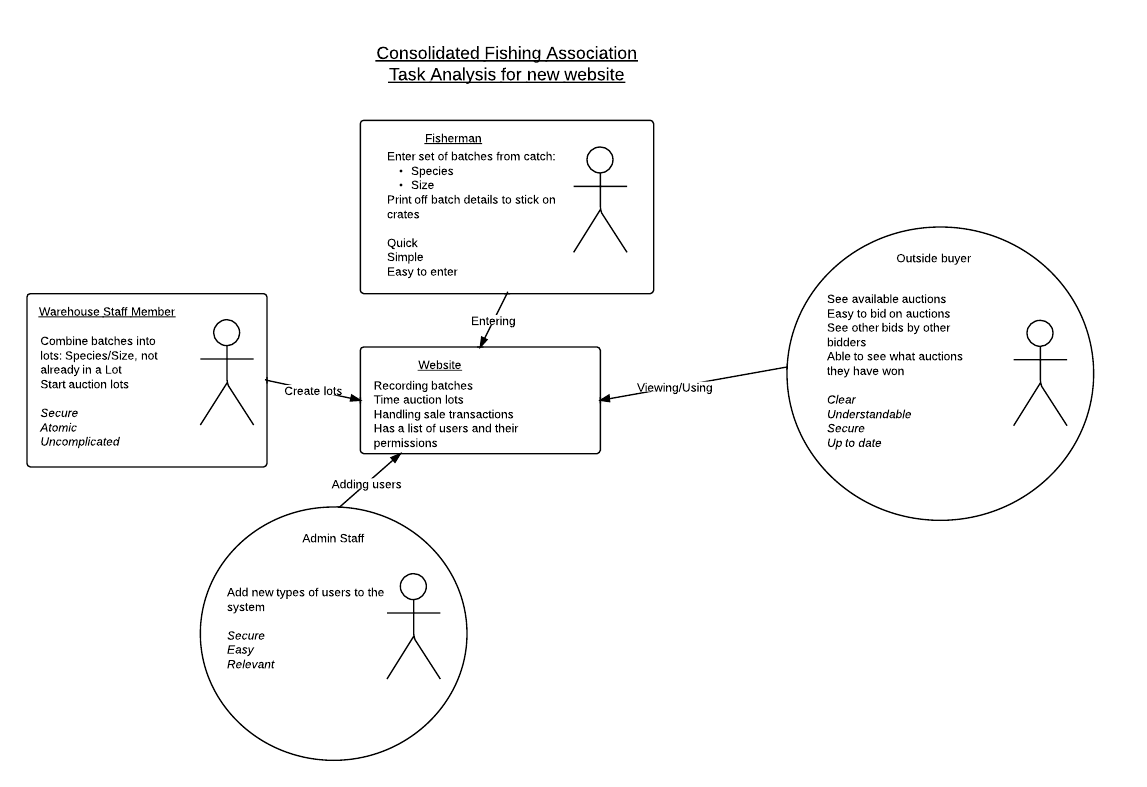
\includegraphics[width=0.8\textwidth]{img/TA-RP1.png}
	\caption{A rich picture to show who the users are and what they require from the system}
\end{figure}
\subsection{Use Case Diagram}
From further  examination of the functional requirements, I found it useful to draft up a Use Case diagram, displaying the basic needs of each individual person who will be using the application, and what might be needed for them to accept this application into their daily routine.

\begin{figure}[H]
	\centering
	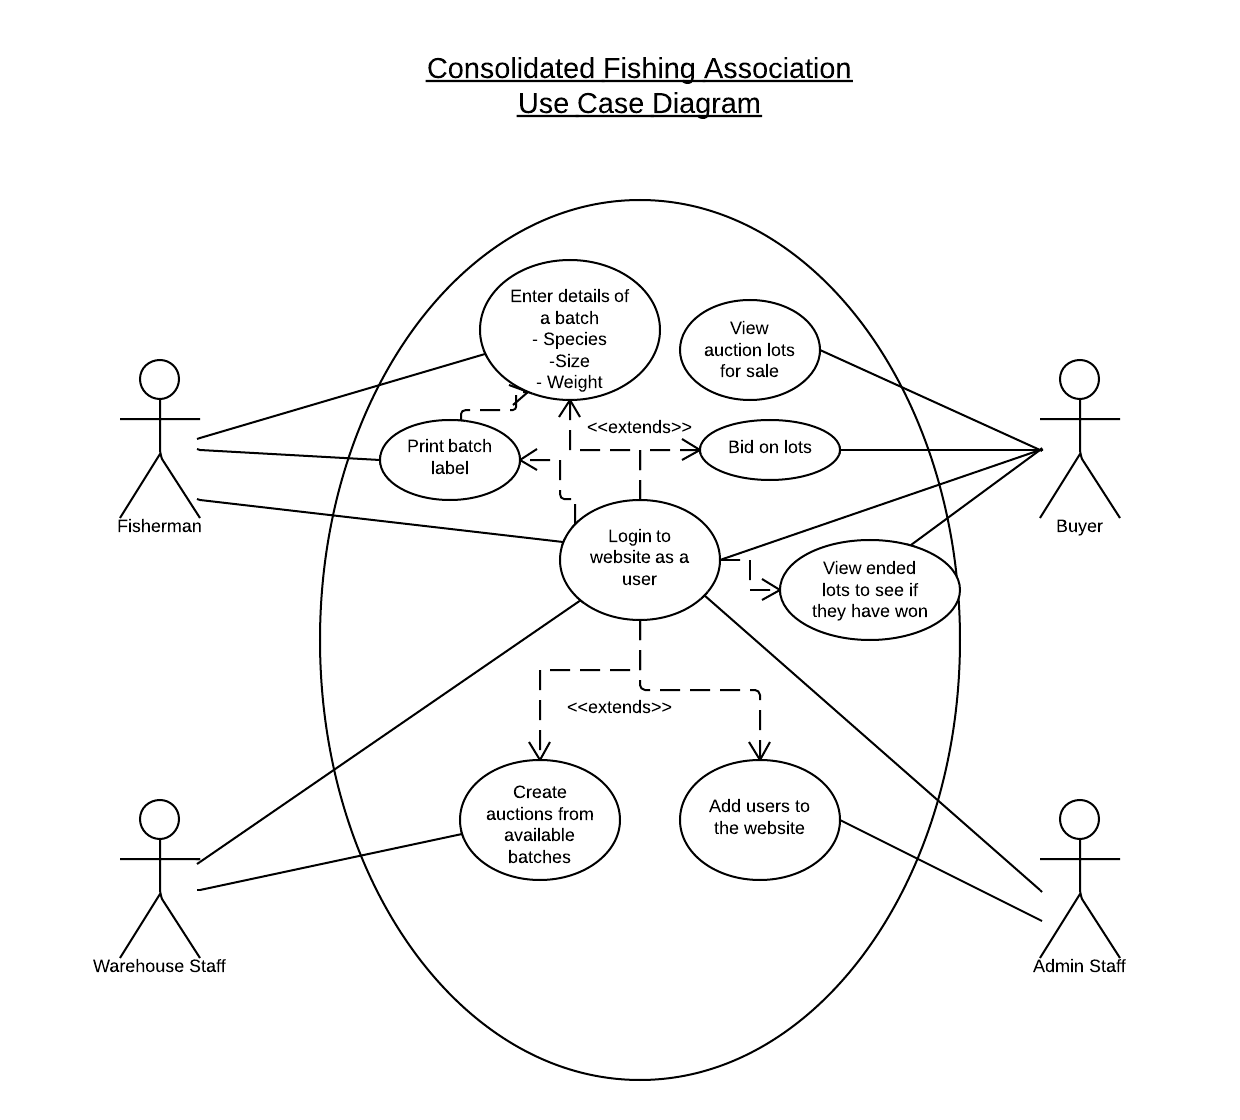
\includegraphics[width=0.8\textwidth]{img/TA-UCD1.png}
	\caption{A Use Case diagram to visually represent each users need and how they are shared or separate from one another.}
\end{figure}

As seen from the figure, each user is required to log in to the system, where they are each presented with their own different options of progressing from there, based on their particular needs and expectations on the website. This leads up to helping with the design decisions of how to best make the website design later, in order to accommodate for each different type of user, and provide them with the services they need on the same platform, without giving them access to everything or nothing.
If a user was provided with more than they needed, it would confuse them. If they were to be presented with less than they expected, they could get highly frustrated. Using this Use Case diagram, I can clearly see how each user will expect the application to look for them, and cater to their needs accordingly.

\subsection{Data flow}
When dealing with a website that handles data of different types of users, I found it good to create a diagram to represent the flow of data in the application. This ignores why or how exactly the data flows this way, and focuses on the actual flow of the data. From where does it start and where does it go to, and what is in the data. 

Doing this helped me get an idea of what the finished product would look like in the underlying data structure, and also imagine each type of user interacting with the program, and how they themselves would expect the flow of data to be on the website as a whole.
\begin{figure}[H]
	\centering
	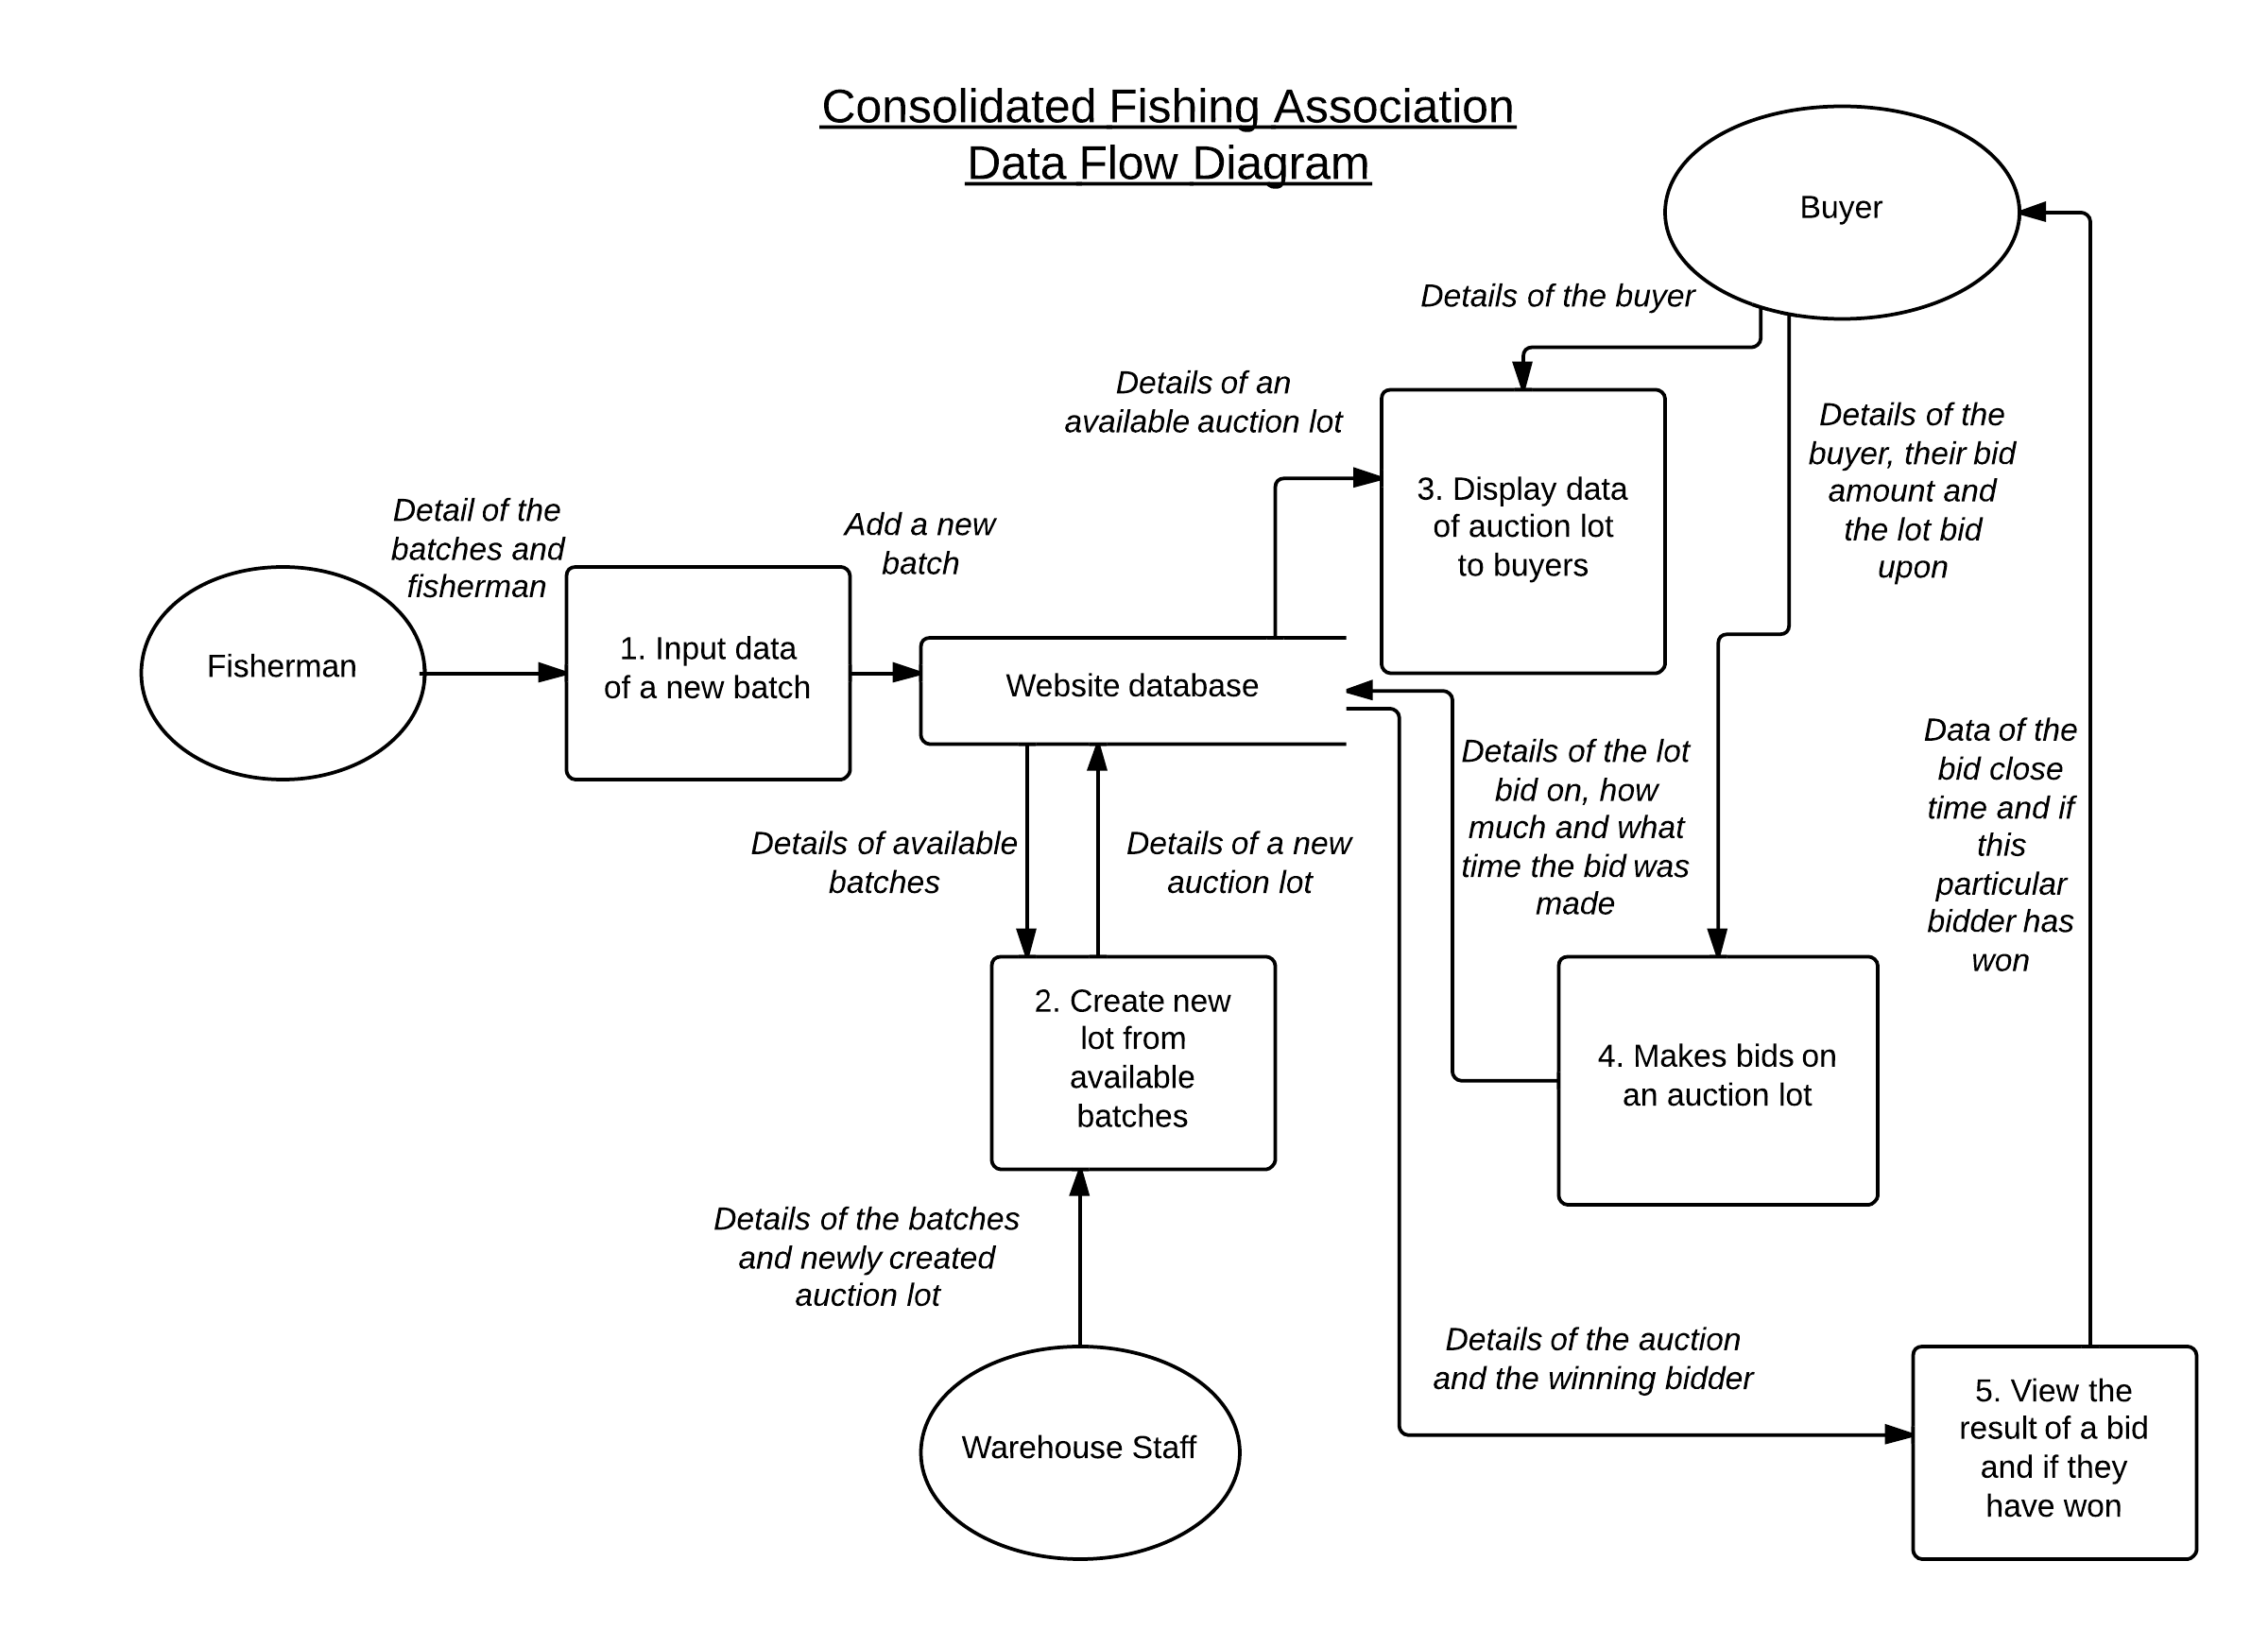
\includegraphics[width=0.8\textwidth]{img/TA-DFD-Transaction.png}
	\caption{The flow of data, as it enters the application from the Fisherman and where it travels to for each user to see.}
\end{figure}
This next figure displays the flow of data for registering a new member and the data flow in order to instate them as a member of the website with the correct access they require for their needs.
\begin{figure}[H]
	\centering
	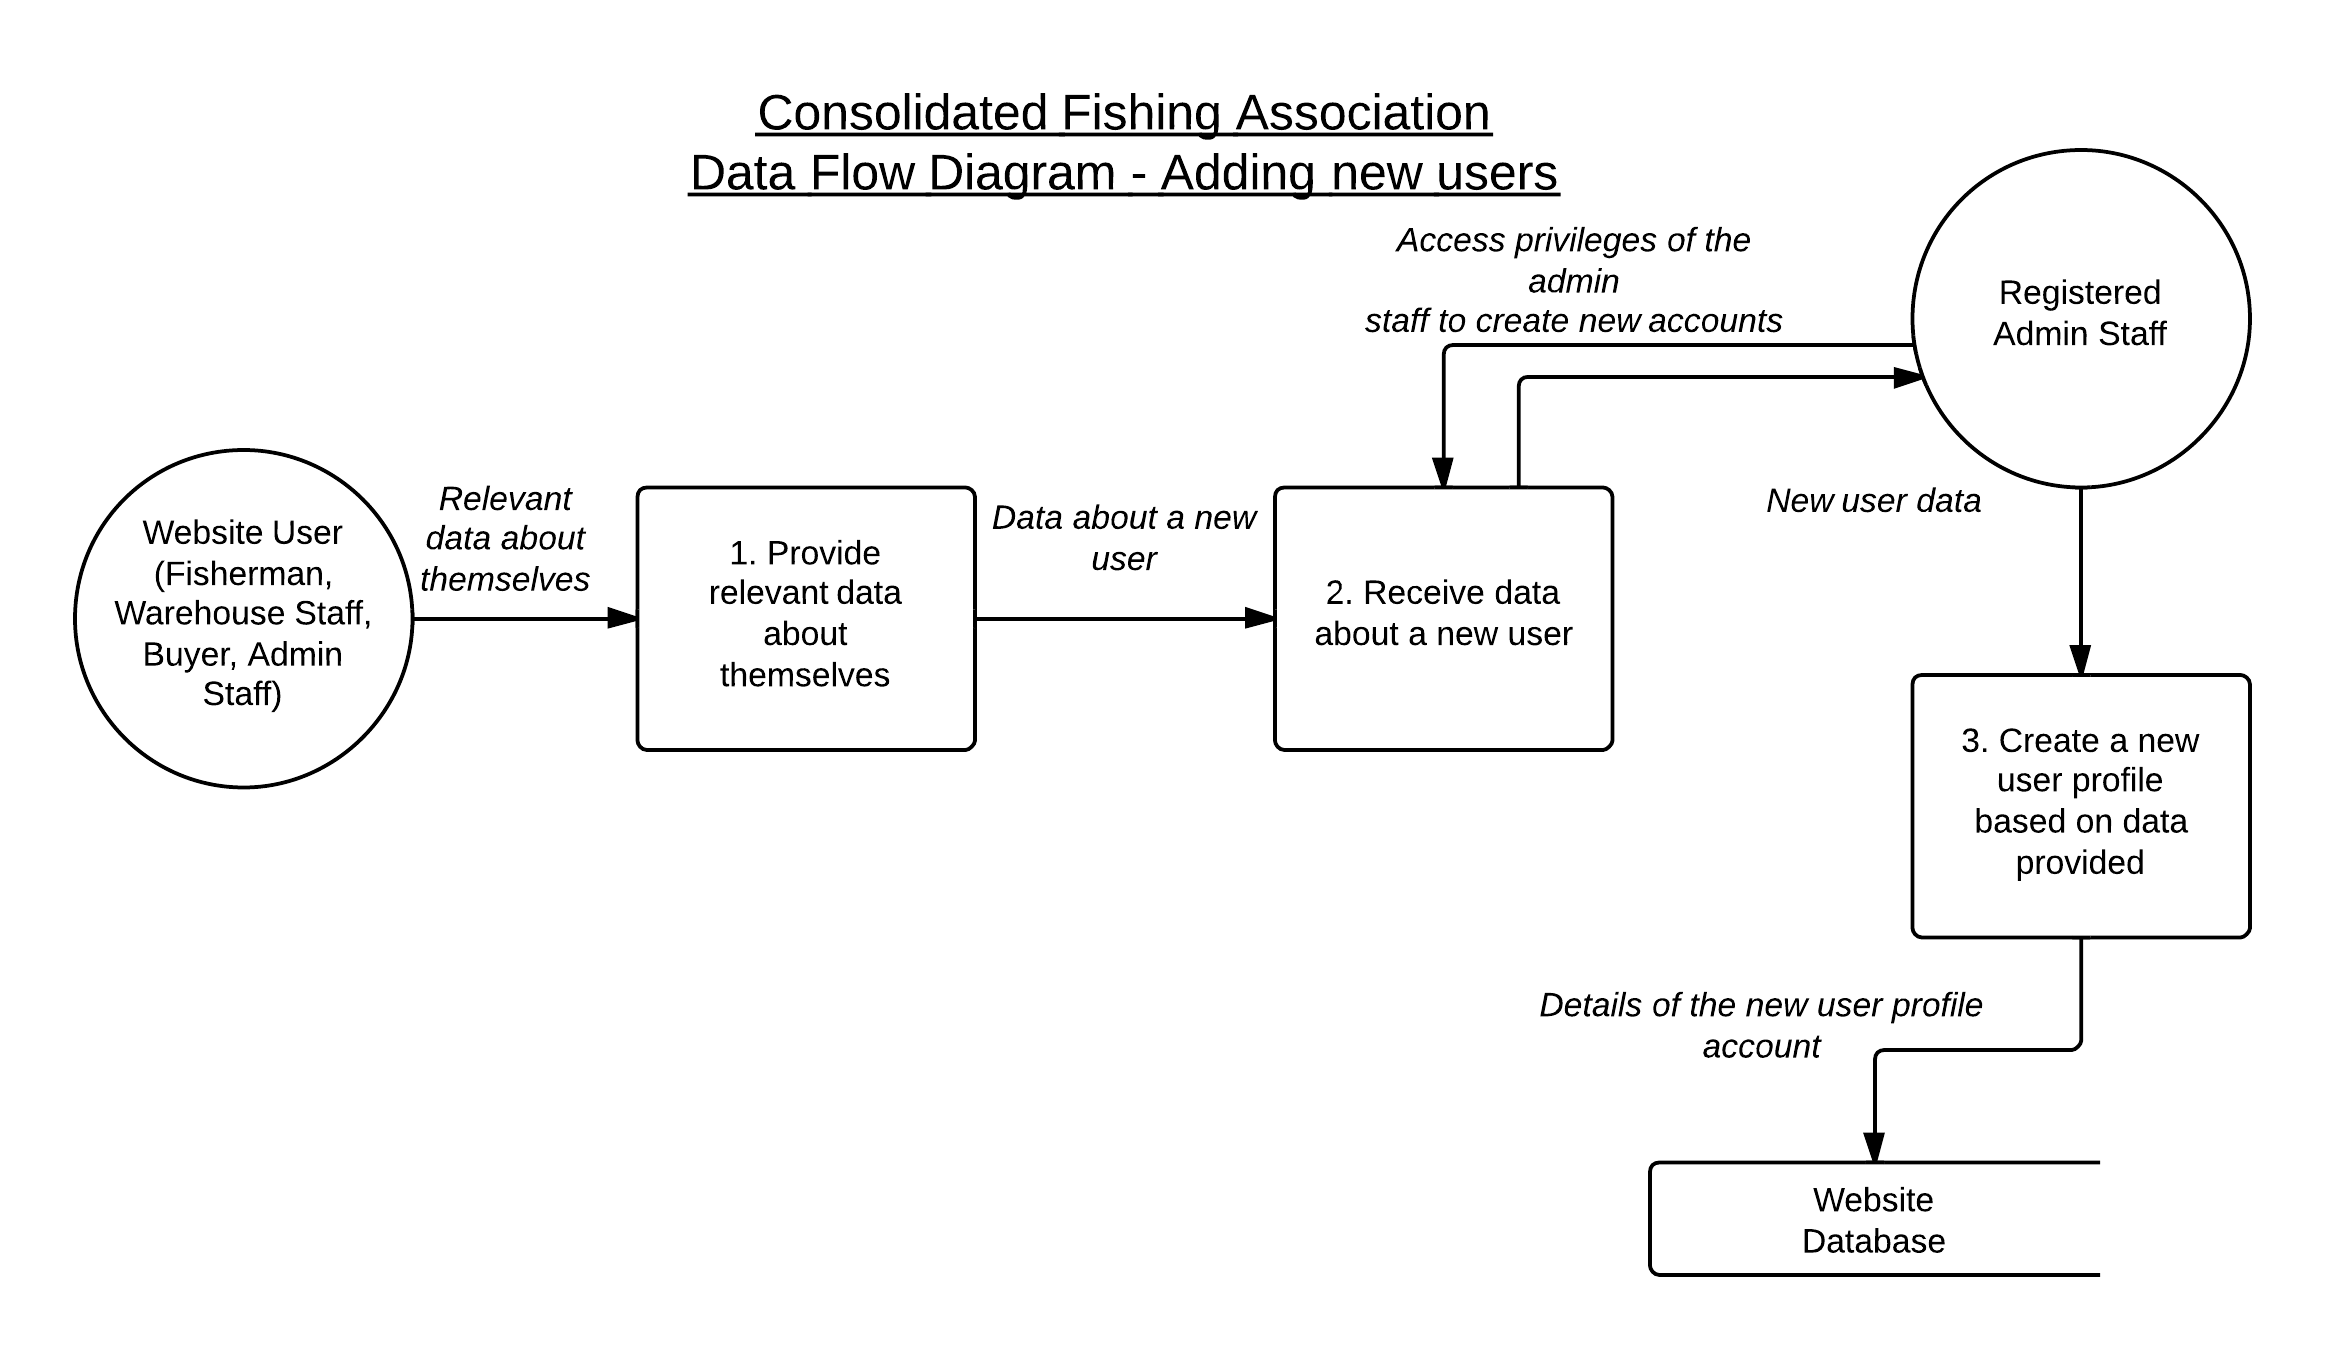
\includegraphics[width=0.7\textwidth]{img/TA-DFD-User.png}
	\caption{The flow of data, provided by the new user and passing through the application to instate them as a member on the website.}
\end{figure}

\subsection{State Transitions}
There are also a number of states that the user and the website can be in, that must be processed in order for all of the tasks that each member of the website wants to perform can be executed correctly. To demonstrate, here are some state diagrams, showing how the real world uses of the website affect the state of the website for other members of it, and how they are able to reach their needs. These diagrams also touch upon how a user of a particular type and view and use the website.

\begin{figure}[H]
	\centering
	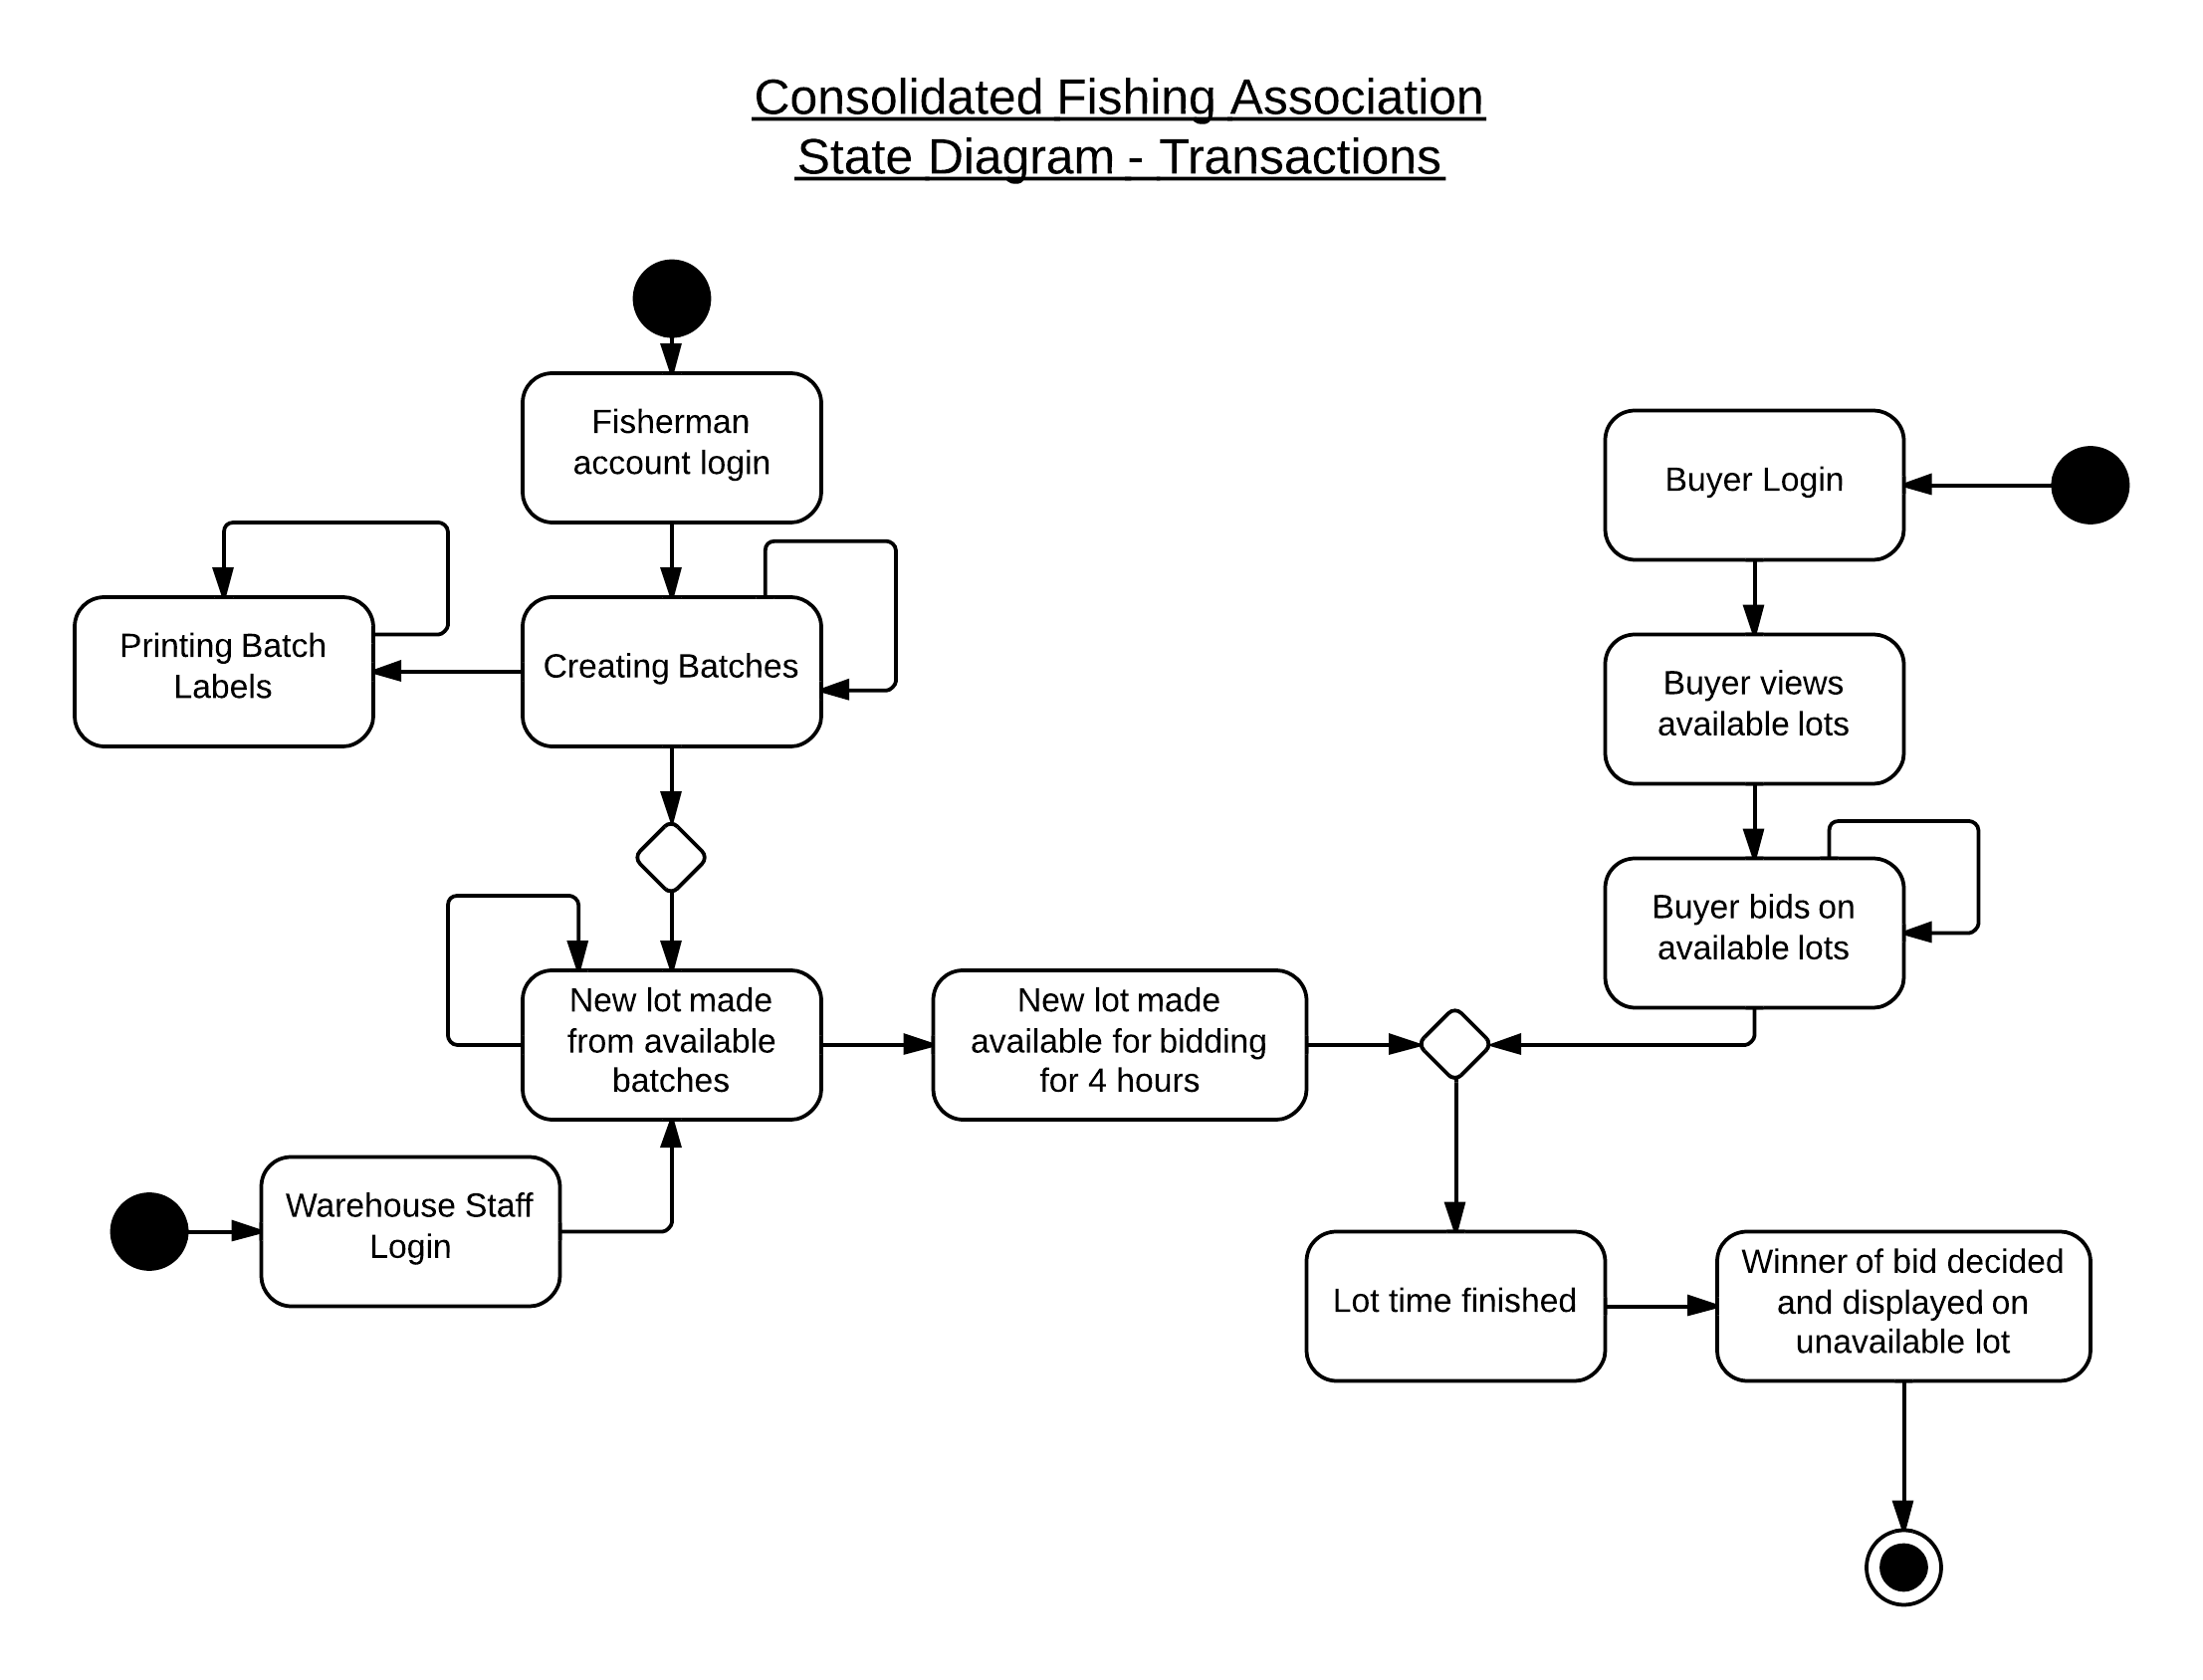
\includegraphics[width=0.7\textwidth]{img/TA-SD-Batches.png}
	\caption{The states of the process of users using the website, from the fish batches being entered into the website, to the state of fish being sold.}
\end{figure}

\begin{figure}[H]
	\centering
	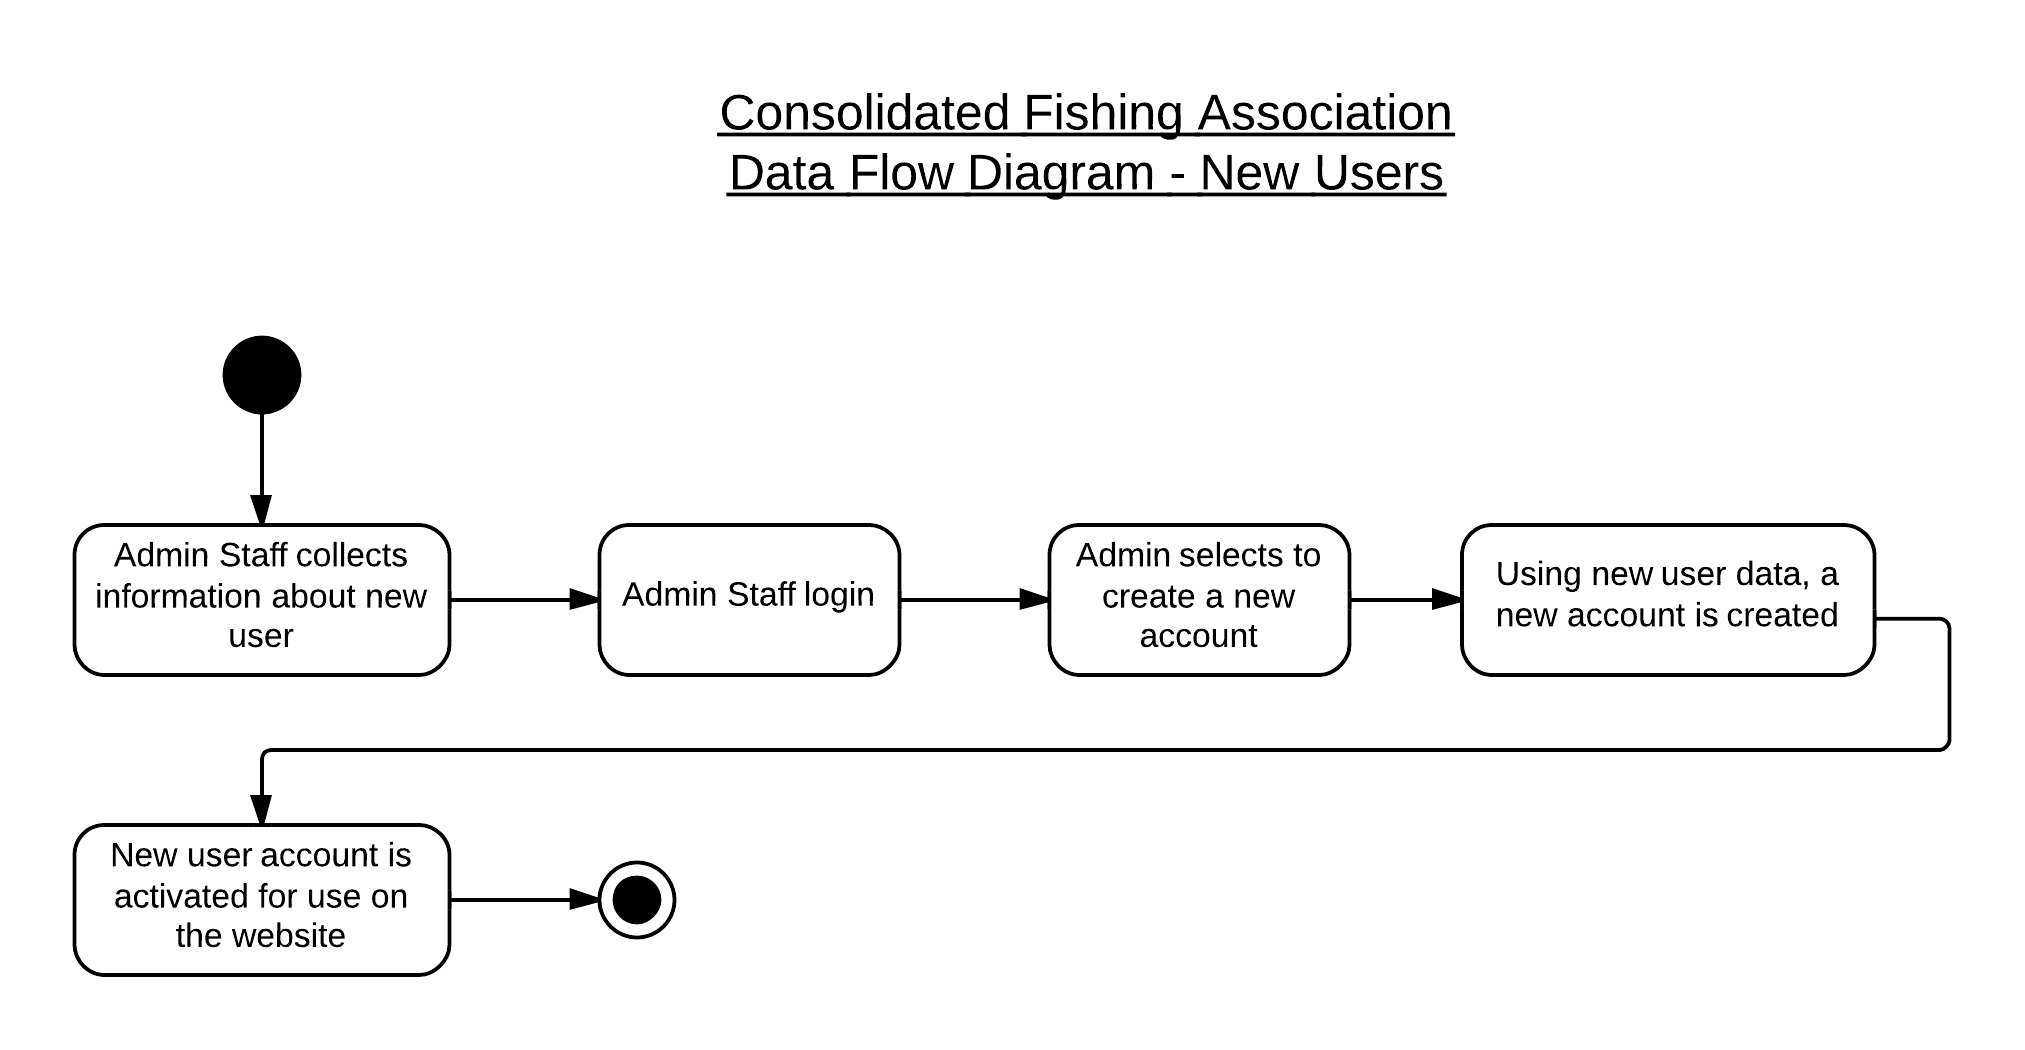
\includegraphics[width=0.7\textwidth]{img/TA-SD-Users.png}
	\caption{The states of a new account creation for the website.}
\end{figure}

Through the analysis of the tasks a user wishes to perform with the website, as set out by the requirements specification, I had a clear idea of exactly what and how the application should function. The next stage was to design the website in such a way that these expectations could be met, and give the users the best and simplest interaction with the website as possible. With the diagrams to refer to a later points, they give a solid understanding of how I had to balance the design of the website with it's usability for the target users.

%----------------------------------------------------------------------------------------
%	DESIGN
%----------------------------------------------------------------------------------------

\section{Design}
\subsection{Interaction Design}
\subsection{Navigation}


%----------------------------------------------------------------------------------------
%	PROTOTYPE - Link + Brief info
%----------------------------------------------------------------------------------------

\section{Prototype}

%----------------------------------------------------------------------------------------
%	Shneiderman's 8 GOLDERN RULES
%----------------------------------------------------------------------------------------

\section{Shneiderman’s 8 Golden Rules}

%----------------------------------------------------------------------------------------
\clearpage

%----------------------------------------------------------------------------------------
%	REFERENCES
%----------------------------------------------------------------------------------------

\begin{thebibliography}{1}

\bibitem{assignment} N. Hardy, "Fishing Association Project Requirements Specification", CS22310 Assignment 2014, 17th March 2014

%\bibitem{w3c} W3schools.com (Accessed 18/04/2014) JavaScript Tutorial [Online]. Available: http://www.w3schools.com/js/



\end{thebibliography}


\end{document}


